\documentclass[12pt]{amsart}

\addtolength{\hoffset}{-2.25cm}
\addtolength{\textwidth}{4.5cm}
\addtolength{\voffset}{-2.5cm}
\addtolength{\textheight}{5cm}
\setlength{\parskip}{0pt}
\setlength{\parindent}{15pt}
\usepackage[ngerman]{datetime}

\usepackage{amsthm}
\usepackage{amsmath}
\usepackage{amssymb}
\usepackage[colorlinks = true, linkcolor = black, citecolor = black, final]{hyperref}

\usepackage{graphicx}
\usepackage{multicol}
\usepackage{ marvosym }
\usepackage{wasysym}
\usepackage{tikz}
\usetikzlibrary{patterns}

\newcommand{\ds}{\displaystyle}
\DeclareMathOperator{\sech}{sech}


\setlength{\parindent}{0in}

\pagestyle{empty}

\begin{document}

\thispagestyle{empty}

{\scshape \today} \hfill {\scshape \large Ziel-Definition} \hfill {\scshape Bachelor These}
 
\smallskip

\hrule

\bigskip

\section*{{\bf Titel/Aufgabenstellung}}
\begin{itemize}
\item[(15.Juni)] Die Automatisierung des Knowledge Managements der fachlichen Software-Architektur in einem X-Team mit agiler Organisationsstruktur
\item[(22.Juni)]Untersuchung der Kopplung in einer Aws-Ressourcen Microservice-Landschaft mit Hilfe einer Graph-Datenbank
\item Untersuchung der Kopplung in einer Aws-Ressourcen Microservice-Landschaft 
\bigskip
\item[(30.Juni)] Untersuchung der Kopplung in einer Aws-Ressourcen Microservice-Landschaft mit agiler Organisationsstruktur
\item[(11.Juli)] Ist schwerfällige Kommunikation in einer agilen Organisationsstruktur ein Symptom für zu hoher Kopplung in einer Microservice Landschaft.
\textbf{\item[(12.Juli)] Schwerfällige Kommunikation als Symptom für zu hohe Kopplung in einer Microservice Landschaft.}
\end{itemize}

\bigskip



\bigskip
\section*{{\bf Einleitung - Problem}}
Das Projekt Deapsee in einem Unternemhem soll die Monlitische und schwerfällige Software landschaft in modulare leichter wartbare Microservice Landschaft verwandeln. H

\bigskip


\section*{{\bf Fragen}}

\medskip

\begin{enumerate}

\item Was ist das Problem?
\item Grenzwerte betrachten?
\item Wo können Probleme Auftauchen
\item Definitionen der Bestandteile 
\item Kopplung
\item Microservice-Landschaf
\item Daten?
\begin{itemize}
    \item wo kommen die Daten her? 
    \item wie müssen die Daten beschaffen sein?
    \item gibt es Marker zur Identifikation der Kopplung?
    \item Wie bekomme ich die Daten der X-Team?
    \item Wie die Daten aufbereiten um eine Analyse durchführen zu könne?
\end{itemize}
\item 
\item Wie wird das System genutzt...?
\item 


\end{enumerate}




\medskip

\newpage

\begin{center}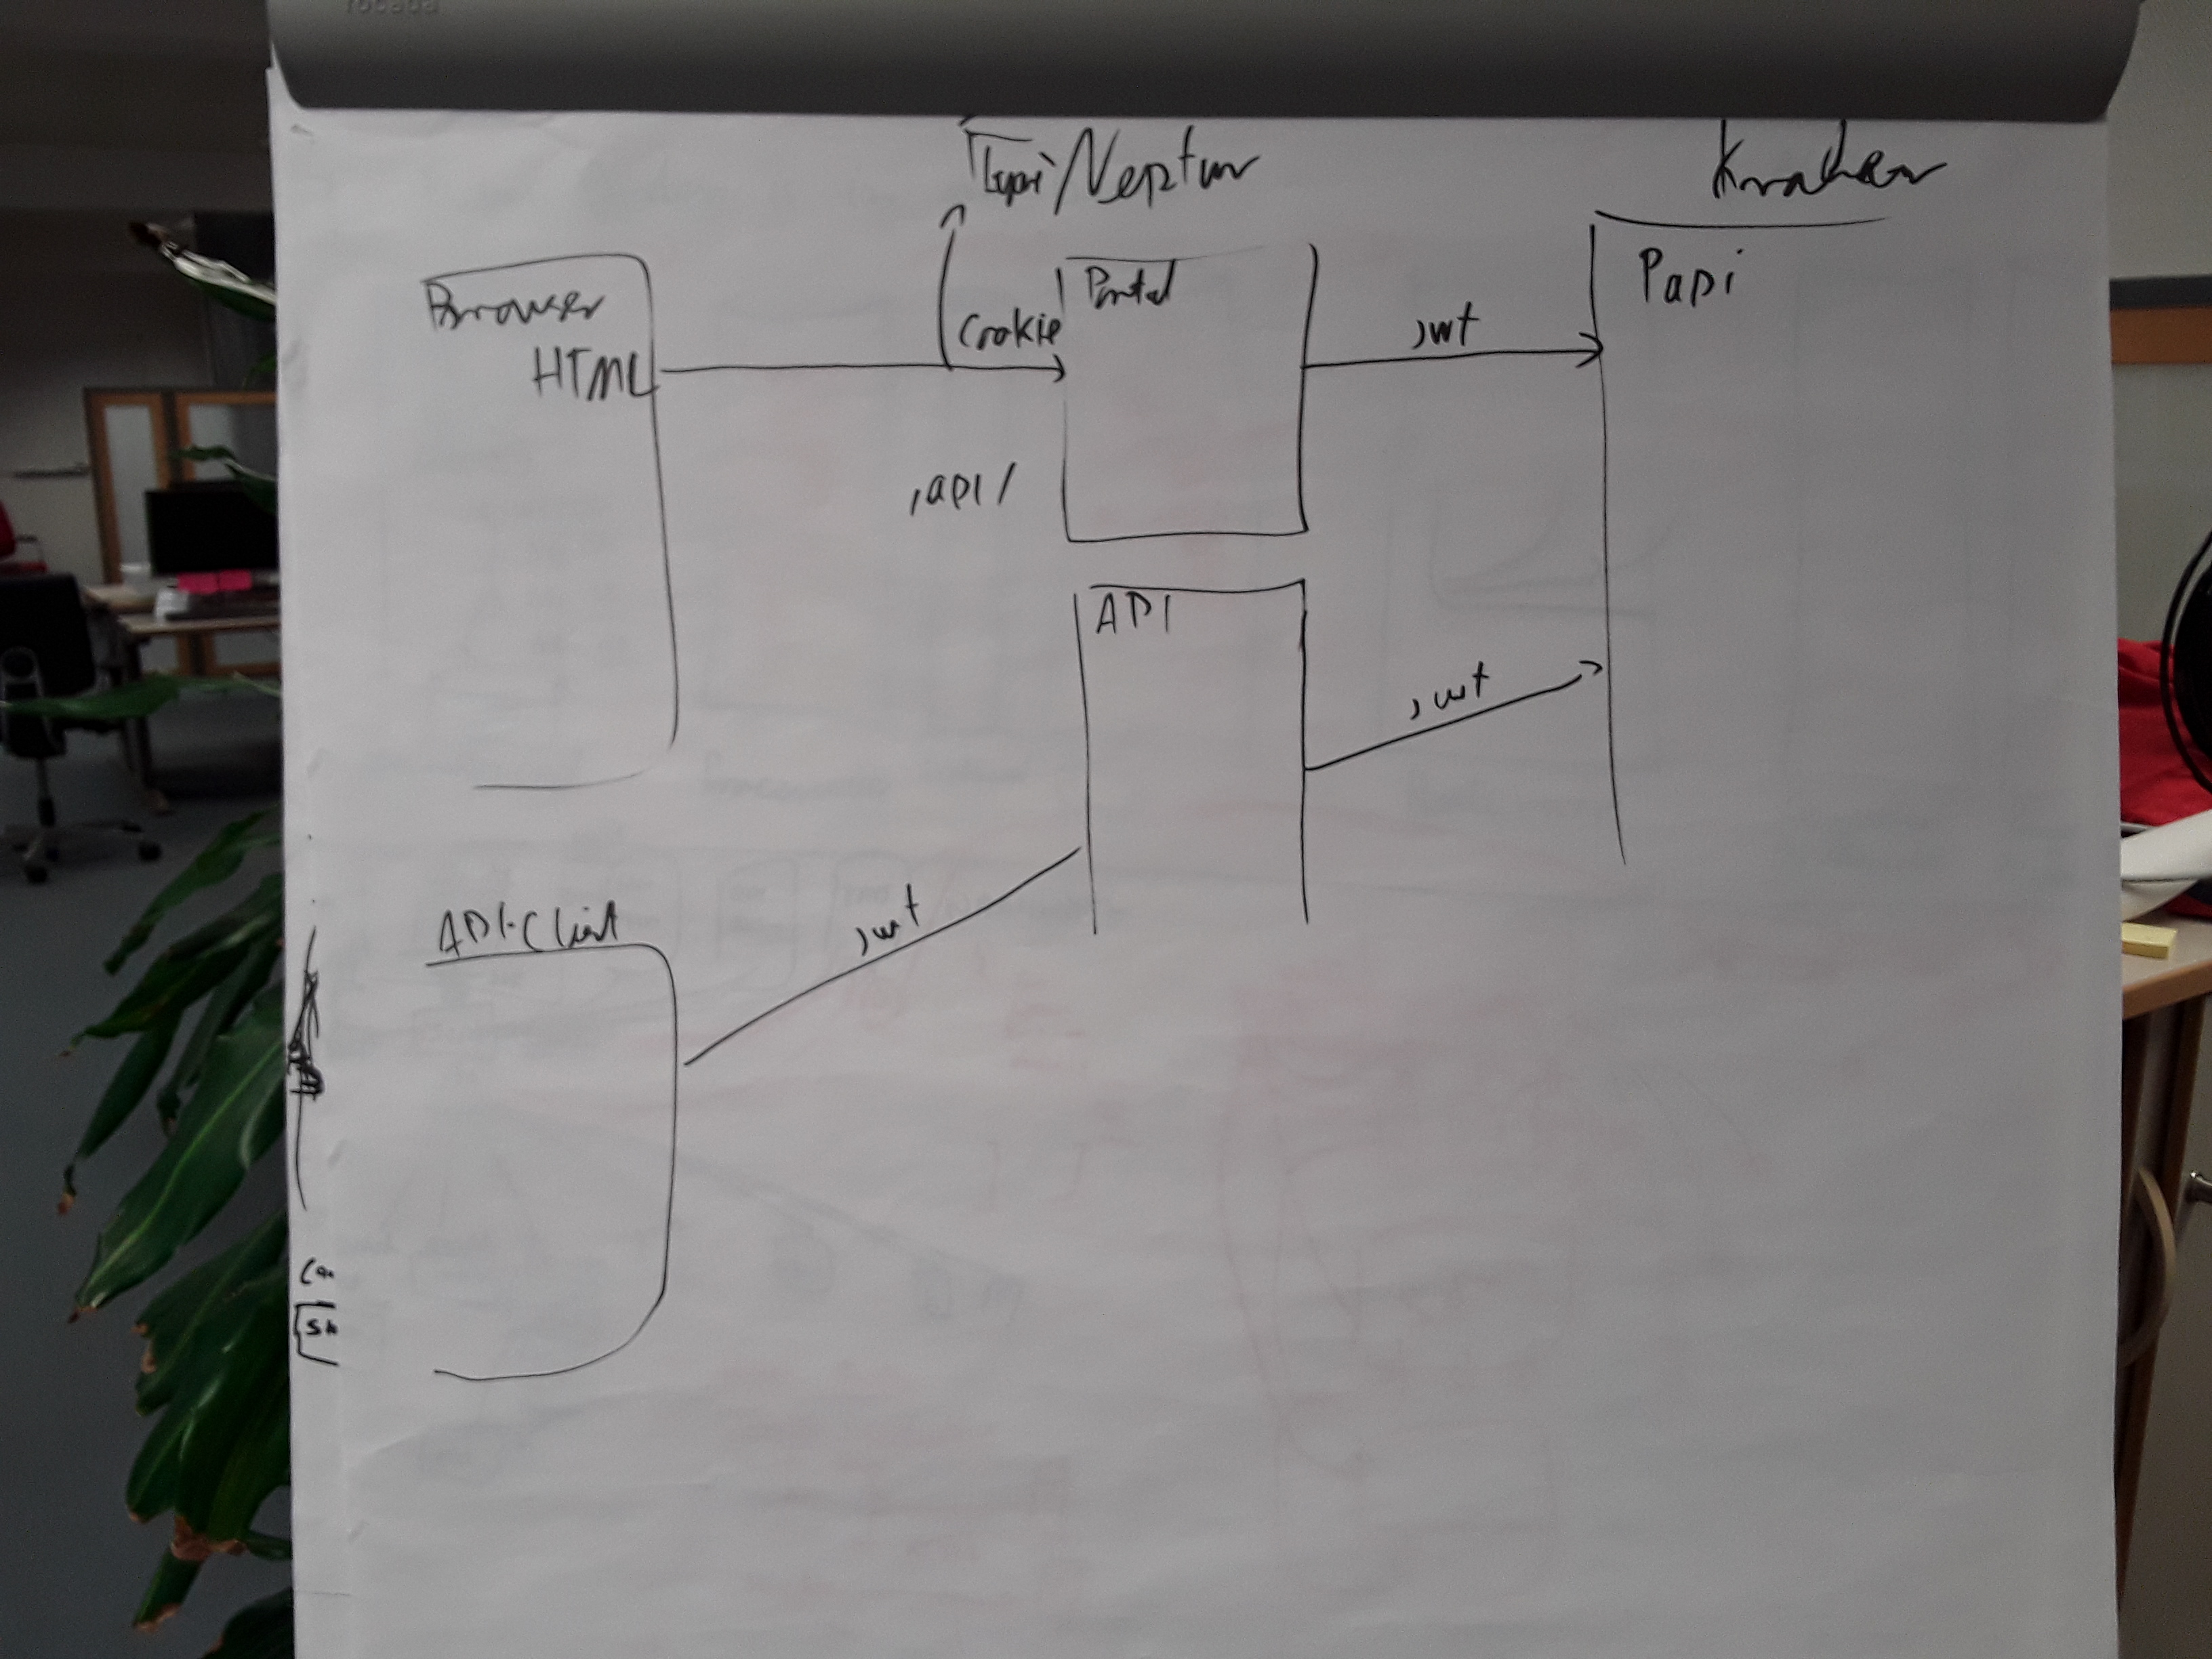
\includegraphics[scale = 0.14]{whith-board _1.jpg}\end{center}

\end{document}